{
\cleardoublepage
\let\clearpage\relax
\chapter{Overall Architecture and Design}
\section{High-Level System Components}

The proposed \acrshort{hpc} architecture leverages three distinct computational strategies to improve the speed, efficiency, and throughput of \acrshort{pra} quantifications. These approaches address the computational demands of modern \acrshort{pra} by utilizing available hardware resources and parallel computation techniques.

\begin{enumerate}

    \item \textbf{Parallel Computation on Shared Memory:} Implemented primarily for importance measures and uncertainty quantification tasks, this approach utilizes multicore \acrshort{cpu} architectures (e.g., via \acrshort{openmp}) to parallelize computations.
    
    \item \textbf{Task-Parallel Distributed System on Distributed Memory:} This implementation is designed to horizontally scale \acrshort{pra} solvers. Computational tasks including probability estimation, uncertainty analysis, and importance measures are assigned as discrete tasks to independent computational nodes. Tasks are managed via REST \acrshort{api}s interfacing with a distributed task queue, facilitating concurrent task execution.
    
    \item \textbf{Data-Parallel Monte Carlo Probability Estimator:} Specifically developed for probability estimation, this solver turns fault trees into layered graphs that can be simulated in parallel on \acrshort{gpu}s or multicore \acrshort{cpu}s. Millions of random samples of each basic event are generated and bit-packed to reduce memory usage. \acrshort{sycl} kernels then work their way up the layers, combining the results in topological order and use hardware-accelerated pop-count instructions to evaluate the outcome of the gates on the fly.
\end{enumerate}

Collectively, these strategies enable the modernized \acrshort{pra} platform to handle much larger models, compute them faster, and process many more concurrent quantifications than was previously possible.

\subsection{Priority Queues and Active Queue Management Strategies}\label{subsec:priority-aqm}

\subsection{GPU Acceleration and CPU-Multicore Approaches}\label{subsec:gpu-accel}

% \section{A Brief History of PRA Tools}
% \label{sec:history_of_pra_tools}

% Probabilistic Risk Assessment (PRA) has evolved dramatically since its inception in the 1970s, driven both by the growing complexity of nuclear power systems and by substantial leaps in computing technology. Early PRA efforts were primarily focused on relatively small reactor models, typically analyzed with mainframe computers or custom in-house codes. Over time, the field has shifted from batch-oriented, single-CPU environments to desktop-based tools and, more recently, to parallel and cloud-based software poised to exploit high-performance computing (HPC). This section first outlines the motivations for PRA software over the decades and then examines representative PRA tools, culminating in a contemporary view of how evolving hardware, licensing, and operational needs have given rise to the current landscape.

% \subsection{Computing Landscape from the 1970s to the 2020s}

% \paragraph{1970s: Mainframe Computing and Foundational PRA Studies.}
% The seminal Reactor Safety Study (WASH-1400) in the mid-1970s introduced wide-ranging probabilistic techniques for assessing reactor safety. While this study provided a rigorous framework, it also underscored the limitations imposed by mainframe computing resources, which constrained the size of fault trees and event trees that could be analyzed. Early PRA codes, such as PREP and KITT~\cite{vesely_prep_1970,vesely_prep_1997}, operated in these mainframe environments and performed either Monte Carlo or deterministic methods to identify Minimal Cut Sets (MCS) and compute their probabilities.

% \paragraph{1980s--1990s: Transition to Personal Computers.}
% By the 1980s, the expansion of Light Water Reactor (LWR) licensing and the increasing complexity of PRA models led to the introduction of more advanced tools. MOCUS~\cite{Fussell1974MOCUS}, MODULE~\cite{module}, SIGPI~\cite{sigpi}, and RISKMAN~\cite{riskman1,riskman2} are examples of software developed to handle larger fault trees and event trees, shifting computational tasks onto personal computers rather than mainframes. While personal computers substantially reduced hardware costs, early desktop-based PRA tools often suffered from limited memory, slower processors, and rudimentary user interfaces. Nevertheless, this period saw the gradual shift toward stand-alone, desktop-centric PRA applications that offered more intuitive workflows.

% \paragraph{2000s: Emergence of Distributed, Web-Based, and Parallel Solutions.}
% With improving desktop performance and the emergence of web-based applications, more collaborative PRA tools began to appear. At the same time, parallel computing gained traction, particularly within the broader high-performance computing community. In the PRA world, large-scale event tree and fault tree evaluations were beginning to see benefits from multi-core processors and basic clustering. Tools such as SAPHIRE~\cite{saphire1,SAPHIRE,saphire_manual} (stemming from IRRAS~\cite{irras1,irras2}) expanded the usability of PRA for day-to-day licensing work, while CAFTA~\cite{cafta1,cafta2} and RiskSpectrum~\cite{riskspectrum1} catered to utility operators requiring detailed station-specific reliability calculations. While initial HPC-oriented attempts remained limited, the growing push toward distributed architectures signaled the community’s recognition that next-generation PRA problems would benefit greatly from parallel computing paradigms.

% \paragraph{2010s--2020s: Contemporary Large-Scale and GPU-Enabled Paradigms.}
% Continued growth in model complexity—driven by non-LWR reactor designs, multi-hazard considerations, and real-time or near-real-time decision-support needs—further accelerated interest in HPC. During this period, open-source initiatives like SCRAM~\cite{scram} demonstrated how community-driven development could incorporate modern software practices: flexible input formats, automated build pipelines, and expansions for parallel or GPU-based computations. Commercial software packages, including FTREX~\cite{ftrex_manual}, RiskSpectrum, and others, have likewise adapted to multi-core, cluster, and cloud environments, though often in a closed-source manner. Additionally, specialized research frameworks, such as DeRisk~\cite{derisk1,derisk2}, Trilith~\cite{hcl_method}, and HCLA~\cite{hcla_cmd,hcla_web}, illustrate the quest for dynamic or “on-the-fly” risk calculations that can leverage large compute infrastructures.

% \paragraph{Future Trends: Quantum and Fully Homomorphic Encryption.}
% Looking ahead, the community’s interest in real-time risk monitoring, coupled with confidentiality requirements for sensitive nuclear data, suggests that quantum computing and fully homomorphic encryption (FHE) could eventually play a role in PRA. Although these technologies remain at a relatively early research stage, their potential for massively parallel or secure distributed calculations could address future bottlenecks in handling multi-hazard complexities, intricate dependencies, or large multi-reactor sites.

% \subsection{Representative PRA Tools and Their Evolution}

% Over the decades, a multitude of PRA software tools have been created and refined, each representing an effort to address the specific computational and regulatory challenges of its time. Table~\ref{tab:pra_tools_overview} summarizes both legacy and contemporary tools, highlighting their licensing models and typical usage contexts. For example, CAFTA~\cite{cafta1,cafta2}, originally designed for DOS-based personal computers, now integrates with advanced Windows environments. SAPHIRE, supported by the U.S. Nuclear Regulatory Commission (NRC) and maintained by Idaho National Laboratory, evolved from earlier codes (IRRAS~\cite{irras1,irras2}), bridging desktop-based analysis and more recent cloud-deployment patterns.

% Even with the proliferation of PRA tools, many remain proprietary, limiting the community’s ability to incorporate specialized HPC features or novel algorithms. However, the open-source SCRAM~\cite{scram} suite under the GNU GPL and the MIT-licensed OpenPRA initiative mark a shift toward more collaborative development. These open frameworks foster deeper experimentation with parallel algorithms, advanced sampling methods, and dynamic event-tree evaluations—capabilities that can be critical when analyzing complex, multi-hazard scenarios. Through ongoing cross-institutional collaborations, new HPC extensions are regularly introduced, providing the PRA community with means to surmount performance bottlenecks and scale up to multi-million component analyses.

% \subsection{Opportunities and Limitations in Existing Software}

% Despite considerable efforts to modernize PRA tools, a number of core limitations persist:
% \begin{itemize}
% \item \textbf{Limited Parallelization:} Many legacy applications rely on serial or coarse-grained parallel workflows, insufficient for massive concurrency needs.
% \item \textbf{Closed-Source Development:} Proprietary tools restrict user-driven feature enhancements or specialized HPC adaptations, limiting the scope for research innovation.
% \item \textbf{Platform Dependence:} A heavy focus on Windows-based desktop environments can hamper the integration of containerization, cluster-based scheduling, or cloud-native solutions.
% \item \textbf{Model Size Constraints:} Traditional data structures and memory usage patterns, designed for simpler fault trees and event trees, sometimes struggle with multi-hazard, large-scale models that require efficient parallel memory handling.
% \end{itemize}

% Nonetheless, the increasing availability of cloud resources, multi-node clusters, and GPU-accelerated libraries provides fertile ground for next-generation PRA solutions. By embracing these computational frameworks, practitioners can drastically reduce run times for time-sensitive applications, execute large-scale Monte Carlo or dynamic event-tree analyses, and more readily accommodate expansions into multi-hazard or real-time risk monitoring. This synergy between PRA tools and HPC technologies represents a vital frontier for modeling, regulatory oversight, and operational decision support.

% \subsection{Concluding Remarks on Historical Context}

% From the 1970s mainframe era to modern cloud and GPU-enabled paradigms, PRA software has mirrored the evolution of computing technology. Early codes focused on basic MCS extraction and probability evaluation, while current efforts aspire to large-scale, distributed, and fast-turnaround solutions. This trajectory underscores both the promise and the challenges in harnessing HPC for nuclear risk analysis. The subsequent sections will build upon this historical background, highlighting specific gaps in existing software (Section~\ref{sec:gaps_in_existing_software}) and detailing how contemporary developments in parallel architecture, load balancing, and data management can lead to more robust, accurate, and scalable PRA platforms.


\chapter{Designing a Distributed Queuing System}

\section{Worker-Pool and Queue Management Concepts}

The distributed system follows a \emph{publisher–consumer} pattern. In this architecture, a \textbf{publisher} is typically a client-facing service, such as REST \acrshort{api}s, responsible for receiving requests from front-end clients and forwarding these requests to an exchange inside a message broker. A \textbf{message broker} is a middleware system that facilitates communication between publishers and consumers by routing messages.

Within the broker, the \textbf{exchange} component directs each request to an appropriate queue based on the routing key of the request. A \textbf{queue} is a data structure within the broker that temporarily stores messages until they are processed by consumers. Each queue is configured with specific user-defined settings, such as message time-to-live, maximum queue length, and prefetch limits (the maximum number of messages that a consumer can process simultaneously).

A \textbf{scheduler} layer adds service-level metadata to these messages, including priority, delays, and enforces ordering policies such as \acrshort{fifo} or strict priority ordering. \acrshort{fifo} ensures that messages are processed in the order they arrive, while strict priority ordering processes messages based on assigned priority levels. Queues can be marked as durable, enabling recovery of messages in case of broker restarts or failures. Messages can be marked as persistent, guaranteeing delivery despite network or consumer disruptions. Additionally, queues support a \textbf{dead-letter queue} mechanism, a specialized queue that captures undeliverable or failed messages, allowing for subsequent analysis and recovery operations.

A \textbf{consumer} represents any \acrshort{pra} solver instance within the worker pool. The \textbf{worker pool} is essentially a collection of solver processes running on \acrshort{cpu}s, \acrshort{gpu}s, or \acrshort{fpga}s. These consumers connect to their designated queues and consume messages based on prefetch settings. Consumers process each message by retrieving the \acrshort{pra} models and solver parameters from the message body. Then they perform calculations and persist the results in the distributed databases. Upon successful completion, they send an \textbf{acknowledgement}, a confirmation message indicating successful processing, back to the broker, marking the message as processed.

The broker implements idempotent operations, meaning duplicate or repeated actions are processed only once. For example, if the user repeatedly attempts to create a queue, the broker will create the queue once and ignore the rest of the repeated commands. Finally, both publishers and consumers send periodic heartbeats, regular signals or pings, to the broker to ensure the active status of these components. These heartbeats allow the developers to monitor service availability and manage the health of the distributed system. Figure \ref{fig:worker-pool-queue-management} shows a basic publisher-consumer workflow of a message broker.

\begin{figure}[h]
  \centering
  \begin{tikzpicture}[
      scale=0.7,
      >=stealth,
      box/.style={draw,rectangle,minimum width=2cm,
                  minimum height=0.8cm,align=center},
      msg/.style={->, thick},
      label/.style={font=\small,draw=none}
    ]
    
    % Message Broker components
    \node[box] (exchange) {Exchange};
    \node[box, right=1.5cm of exchange] (queue) {Queue};
    \node[box, below=0.8cm of queue] (dlq) {Dead-Letter\\Queue};
    
    % Fit node for RabbitMQ Message Broker
    \node[fit=(exchange)(queue)(dlq),
          draw, inner sep=0.3cm, dashed, 
          label={[yshift=0.3cm]\textbf{RabbitMQ}}] (broker) {};
    
    % Publisher and Consumer
    \node[box, left=2cm of exchange] (publisher) {Publisher};
    \node[box, right=1.5cm of queue] (consumer) {Consumer\\(PRA Solver)};
    
    % Draw connections
    \draw[msg] (publisher) -- node[above,label]{requests} (exchange);
    \draw[msg] (exchange) -- node[above,label]{routing} (queue);
    \draw[msg] (queue) -- node[above,label]{deliver} (consumer);
    
    % Failed messages
    \draw[msg] (exchange) |- node[pos=0.25,left,label]{failed} (dlq);
    
  \end{tikzpicture}
  \caption{Publisher-consumer message flow with broker internals.}
  \label{fig:worker-pool-queue-management}
\end{figure}

\section{REST APIs for Parallel Task Coordination}

The platform provides a RESTful \acrshort{api} layer that orchestrates the entire life cycle of \acrshort{pra} quantification tasks, from submission and monitoring to cancellation and result retrieval. An \acrshort{api} is a set of rules that lets different software systems exchange data programmatically over the internet. A RESTful \acrshort{api} implements these rules using standard \acrshort{http} methods (GET, POST, PUT, DELETE) and resource-oriented \acrshort{url}s to ensure stateless communication. The REST \acrshort{api}s handles client authentication and payload validation, translating task definitions (\acrshort{pra} models and solver parameters) into messages dispatched to the publisher component of the distributed system. Upon successful POST, clients receive a unique task identifier, which they use to subscribe to status endpoints to get real-time execution updates (queued, running, completed, failed). Batch submission endpoints accept arrays of quantification tasks with optional metadata for target solver selection (\acrshort{mocus}/\acrshort{bdd}/\acrshort{zdd}/Monte Carlo), priority levels, and estimated resource requirements. Result endpoints expose completed outputs and solver performance metrics in \acrshort{json} format via secure download \acrshort{url}s pointing to the distributed databases. To ensure fair usage, the \acrshort{api}s implement idempotent POST semantics and rate limiting to prevent duplicate requests and resource starvation. Figure \ref{fig:rest-api-architecture} shows a simplified workflow of the REST API layer.

\begin{figure}[h]
  \centering
  \begin{tikzpicture}[
      scale=0.8,
      >=stealth,
      box/.style={draw,rectangle,rounded corners=2pt,minimum width=2.2cm,
                  minimum height=0.8cm,align=center,fill=white,drop shadow},
      apibox/.style={draw,rectangle,rounded corners=3pt,minimum width=2.8cm,
                  minimum height=1cm,align=center,fill=blue!10,drop shadow},
      msg/.style={->, thick},
      label/.style={font=\small,draw=none}
    ]
    
    % Client
    \node[box] (client) {Client};
    
    % REST API Layer with its components
    \node[apibox, right=2cm of client] (api) {RESTful API Layer};
    \node[box, below=0.8cm of api] (auth) {Authentication \& Validation};
    
    % Publisher
    \node[box, right=3cm of api] (publisher) {Publisher};
    
    % Database
    \node[box, below=1cm of publisher] (db) {Distributed Databases};
    
    % Fit node for Backend System
    \node[fit=(api)(auth)(publisher)(db),
          draw, inner sep=0.3cm, dashed, 
          label={[yshift=0.3cm]\textbf{Backend System}}] (platform) {};
    
    % Draw connections
    \draw[msg] (client) -- node[above,label]{POST task} (api);
    \draw[msg] (api) -- node[above,label]{models} (publisher);
    \draw[msg] (api) -- node[below,label]{solver parameters} (publisher);

    % Two-way arrow between API and Auth
    \draw[<->, thick] (api) -- (auth);
    
    % Status monitoring path
    \draw[msg, blue] (api) to[bend right=30] node[above,label] {GET results} (client);
    
    % Database connections
    \draw[msg, blue] (db) -- node[right,xshift=0.8cm,label]{query results} (api);
    
  \end{tikzpicture}
  \caption{Simplified RESTful API architecture for PRA task management.}
  \label{fig:rest-api-architecture}
\end{figure}

\section{Design of the Distributed System}

\subsection{Load Balancing and Scheduling}

The distributed architecture is designed to handle a high volume of concurrent PRA quantification tasks with minimal latency and maximum resource utilization. To achieve this, the system employs containerization and cluster orchestration to distribute workloads across multiple computing nodes, combined with scheduling policies to balance the load. Quantification jobs are managed through a message-queue system that decouples task submission from execution, enabling tasks to be executed in parallel by a pool of workers. The framework statically scales the number of worker instances before launch and assigns each job type to its own queue. This scheduling approach reserves resources for every class of quantification task and enables rapid deployment of additional workers when larger models—or large-scale studies—must be processed. Core strategies include (i) distributing tasks across dedicated queues in a Docker Swarm cluster, (ii) using a multi-queue workload manager, (iii) partitioning complex models into parallel tasks, and (iv) adaptively selecting algorithms for each stage of the analysis. These measures collectively provide efficient load balancing and scheduling for the platform's quantification engine.

\subsection{Distributed Task Scheduling in the Cluster}

The distributed queuing system is structured as two loosely coupled, independently deployable microservices within a mono repository: one implements the publisher service, and the other implements the consumer service. These microservices are then deployed as Docker services across a Docker swarm cluster \cite{Swarm}. The cluster consists of a manager node and multiple worker nodes. The manager node is responsible for orchestrating operations and maintaining the cluster state (e.g., monitoring node health and resource usage), while the workers execute the quantification tasks. Both the backend producer service and the worker (consumer) service are containerized as separate Docker  images. The producer service (running on one or more instances) handles incoming analysis requests. It runs the NestJS-based backend \cite{Documentation} and connects to RabbitMQ \cite{RabbitMQ} and the MongoDB \cite{MongoDB} database, and the worker service encapsulates the scram \cite{scram} quantification engine via its Node.js NAPI \cite{Node} bindings, along with its own RabbitMQ client and database access.

When a user submits a model for quantification (for example, by clicking “Quantify” in the web editor or via a REST API call), an HTTP request with the model data and analysis parameters is sent to the backend (producer) service. To avoid sending large files over the network or through the message queue, the backend stores the model input (OpenPSA MEF XML files \cite{2017OpenPSAMEF}) in the MongoDB database and retains only a document ID. The request is then tagged with metadata including the document ID and the requested analysis type. At this point, a priority level is assigned based on the analysis type or urgency of the task. For instance, a simple point estimate might be treated as high priority, whereas a lengthy uncertainty propagation could be set as lower priority. The producer then serializes the task description including the document ID and priority into a message and enqueues it into a RabbitMQ job queue. RabbitMQ serves as the central task broker – it enables asynchronous handling of potentially thousands of jobs without overloading the web server, and it routes tasks to available workers. If multiple producer instances are running, a Traefik \cite{Traefik} load balancer distributes incoming HTTP requests among them, preventing any single backend instance from becoming a bottleneck and thereby balancing the load at the entry point of the system.

On the execution side, a fleet of worker containers run on the Swarm cluster’s worker nodes to perform the actual model quantifications. The manager node can scale the number of active worker containers up or down (currently up to 128 workers across the cluster) to match the incoming workload demand. Each worker continuously polls the RabbitMQ queue for new jobs. RabbitMQ supports multiple queues, so jobs can be segregated by priority or type, and the workers always draw the highest priority jobs first from their individual queues. Once a worker retrieves a job message, it fetches the corresponding model input data from MongoDB (using the document ID in the message), then invokes the scram engine via the Node.js native addon to perform the quantification. By containerizing the scram engine and associated libraries, the system isolates each task’s execution while allowing it to fully utilize a CPU core (or multiple cores if the engine itself is multi-threaded) on the worker node. After the quantification completes, the worker saves the output (results files, logs, etc.) back to the database, associating them with the same document ID for later retrieval. It then sends an acknowledgment to RabbitMQ so that the message is removed from the queue. The platform uses RabbitMQ’s manual acknowledgment mechanism: a task message is only cleared from the queue when a worker signals successful completion. If a worker crashes or fails before finishing, the lack of acknowledgment causes RabbitMQ to automatically re-queue the task, making it available for another worker to pick up. \emph{Figure~\ref{fig:distributed-workflow}} illustrates this distributed workflow: multiple producers accept user requests and queue tasks, and a pool of workers on the cluster consume tasks, quantify and return results.

\begin{figure}[h!]
  \includesvg[width=\textwidth]{4_proposed_solution/dist_queues/figures/distributed_workflow.svg}
  \caption{Distributed task workflow.}
  \label{fig:distributed-workflow}
\end{figure}

\subsection{Multi-Queue Workload Management}
\label{subsec:multi-queue}

The system currently employs a multi-queue architecture that routes requests according to solver execution mode. The worker replicas are statically scaled up (or down), so the cluster cannot dynamically reallocate computational resources among queues. Hence, priority-based routing is not available. Only intra-queue priorities are ensured, meaning higher-priority messages within a queue are processed before lower-priority ones. All queues are hosted in the same RabbitMQ broker, but each provides messages to a distinct worker deployment and calls a different execution pathway inside the cluster.

\paragraph{Queue type~1: API–Model jobs}
This type of queue is used when a client sends an \textsc{http} \texttt{POST} request to \texttt{/quantify} endpoint. The request contains the PRA model in Base64 form (the payload is an OpenPSA MEF XML file, converted to a single Base64 string) together with the chosen solver name (\texttt{scram-bdd}, \texttt{scram-mocus}, \texttt{scram-mc} etc.) and any run parameters. The producer service stores the raw model in MongoDB, inserts the \texttt{model id} along with solver parameters into a JSON task document, and publishes that document to the queue.  A pool of \texttt{model worker} containers subscribes exclusively to this queue.

Each worker:

\begin{enumerate}
  \item Retrieves the task, downloads the model blob from MongoDB, and
        writes it to a temporary file inside the container.
  \item Invokes the designated solver on that file.
  \item Persists the results back to the database and acknowledges the message.
\end{enumerate}

Since the model travels with the message, these jobs are fully self-contained and the cluster does not require shared storage.

\paragraph{Queue~2: API–Exec jobs}
When the client prefers not to embed the PRA model in the request payload, the solver can be invoked as a shell command within a working directory that already contains the input files. In this case, the client sends an HTTP \texttt{POST} request to the \texttt{/execute} endpoint that specifies:

\begin{itemize}
  \item \texttt{workdir} – the absolute path visible on the cluster where the model files reside.
  \item \texttt{cmdline} – the exact tool invocation, identical to how the user would call it on a login node (e.g.\
  \verb|scram --mocus --mcub ft-310.xml|).
\end{itemize}

The producer wraps these two strings in a task document and publishes it
to the queue. A separate deployment of \texttt{exec worker} containers subscribes to this queue; each worker simply change directories into \texttt{workdir} and executes the given command under a limited access shell. This design keeps large input datasets out of the message queues and databases.

\subsection{Model Partitioning for Parallel Execution}

In addition to managing discrete jobs, the quantification engine employs model-specific partitioning strategies to leverage parallelism within a single large analysis. Complex PRA models – notably, large event trees with many branching sequences or scenarios that each depend on fault tree evaluations – are broken down into smaller sub-tasks that can be solved concurrently. Rather than treating a monolithic model as one giant quantification problem, the system identifies independent submodels (subtrees of the overall logic) and distributes those as separate jobs to the cluster. For example, consider an event tree analysis that involves hundreds of linked fault trees (one fault tree for each sequence or safety function outcome). Instead of quantifying each sequence serially, the platform treats each fault tree as an independent quantification task. All fault trees can then be processed in parallel across the distributed workers, each producing a failure probability or cut set result for its respective portion of the event tree. Once all these parallel computations are complete, a post-processing step aggregates the results: the event tree logic is applied to combine the sequence-level probabilities (or other metrics) into an overall result, which is then reported to the user as a single coherent output. This divide-and-conquer strategy acts as a pre-processing (decomposition) and post-processing (recomposition) workflow that enables the handling of extremely complex models which would be infeasible to solve in a single thread or single process. By performing dozens or hundreds of sub-calculations simultaneously, the system can significantly reduce the wall-clock time for quantifying large-scale PRA models.

One advantage of this partitioned approach is that the user can obtain interim results or a rough overview quickly, even if the full analysis is intricate. Because the most critical sub-tasks can be prioritized or because partial results become available as sub-tasks finish, the system could provide a preliminary risk estimate after the first wave of subtrees is solved, then refine that estimate as the remaining subtrees complete. In practice, the initial results might be less precise (for instance, based on a subset of scenarios or a simplified combination of outcomes), but as more computational resources come online or as more sub-tasks finish, the overall result converges to the high-accuracy answer. This means the platform can deliver a quick assessment to analysts (useful for time-sensitive decision support) and then follow up with increasingly accurate results as computation continues, effectively trading off accuracy and time. 

Moreover, the engine takes an adaptive algorithmic approach during quantification to optimize both accuracy and performance for each sub-task. Different solving algorithms excel under different conditions, so the engine can choose the most appropriate method on a per-subtask basis. For example, the MOCUS algorithm (which enumerates minimal cut sets) is very fast for low-probability scenarios but tends to lose accuracy (overestimating the top event probability) in scenarios with high component failure probabilities, due to the limitations of the rare-event approximation. On the other hand, binary decision diagram (BDD) based methods yield exact results even with higher failure probabilities but can be slower or more memory-intensive for very large logic structures. To capitalize on these strengths, the system can automatically apply a BDD-based quantification for portions of the model that involve high probability events or densely interdependent logic, while using MOCUS (potentially with approximations like the min-cut upper bound, MCUB) for other portions. In the previous example of an event tree with many fault trees, this might mean using a BDD solver for a particular fault tree known to have high-risk (high probability) contributors, and using the faster cut-set solver for fault trees in which the rare-event assumption holds. By mixing algorithms in this way, each sub-task is solved with the method best suited to its characteristics, ensuring that the final results are accurate without incurring unnecessary computational overhead.

\subsection{Handling Shared Subtrees in Distributed Memory} A particular challenge in the parallel decomposition of a PRA model is handling shared subtrees in a distributed memory environment. Shared subtrees occur when different parts of a model require the evaluation of an identical sub-model. For instance, in an event tree analysis, multiple accident sequences might involve the same mitigating system fault tree; similarly, in a large fault tree, two separate top events or portions of the logic might include a common subtree (a repeated gate structure or module). In a single-process solver, such common substructures can be computed once and reused internally to save time. However, in a distributed system each worker operates with its own memory and state, so without coordination, the same subtree could be sent to two different workers and thus be quantified twice in isolation. This would waste computational effort. The scheduling strategy avoids this by ensuring that each unique subtree is solved only once.

Before distributing tasks, the system identifies any duplicate or shared subtrees among the jobs. Rather than dispatching redundant tasks, it will assign the computation of a shared subtree to a single designated worker and hold or coordinate the dependent tasks until that worker produces the result. For example, if two event tree sequences both require the fault tree FT1, the scheduler will create a task for quantifying FT1 only once. The first sequence that needs FT1 triggers the FT1 task to be queued; the second sequence’s task sees that FT1 is already in progress (or completed) and will not generate a duplicate FT1 job. When the one worker finishes solving FT1, its results (cut sets, intermediate BDD, or failure probability) are stored in a common repository – in this case, the MongoDB database – and indexed by an identifier (such as the subtree’s ID). Then, any pending computations that depend on that subtree can retrieve the result and proceed without recomputing it.

In the event tree scenario, once fault tree FT1’s probability is known, it can be plugged into all sequences that require it, and those sequences’ quantifications can continue or be finalized. This mechanism effectively simulates a shared memory for that piece of data: although the cluster is distributed, the intermediate result is made available to all relevant processes through the centralized database. During the aggregation phase, the coordinator (a processed job service dedicated for aggregation process) combines the unique results from each subtree to form the overall outcome. This approach does require careful scheduling logic – workers might need to wait for a shared dependency to be solved by another worker. This implementation is essential for large PRA models, where repeated subtrees are prevalent.

\section{Implementation of the Distributed System}

\subsection{Software Stack and Technology Selection}

\textbf{NestJS, TypeScript and RabbitMQ:} The platform uses NestJS, a Node.js based framework, with TypeScript \cite{starting} for its web services. TypeScript’s static typing reduces runtime errors by validating the request and response payloads at compile time. NestJS provides a modular architecture with dependency injection and out-of-the-box support for microservices that simplifies building structured REST API based services. RabbitMQ provides all the advanced features of a message broker at no cost, while ensuring high-throughput and low latency for job processing.

\textbf{MongoDB:} Distributed MongoDB databases are used for persisting PRA models and results. MongoDB was selected for its flexible document schema and horizontal scalability (via sharding). This schema flexibility is ideal for PRA data (e.g., fault trees, event trees, Bayesian networks, etc.) which can have heterogeneous structures.

\textbf{C++ Quantification Engine (scram) and NAPI:} The quantification tasks are handled by the scram engine, written in C++. To integrate this native engine with the TypeScript language, OpenPRA employs Node’s N-API (Node Addon API). N-API bridges the TypeScript and C++ layers by compiling scram’s functions into a Node.js module, allowing the TypeScript code to invoke C++ quantification methods directly. This approach offers the speed of optimized C++ code while keeping the high-level logic in TypeScript, and abstracts away the complexity of the C++ codebase from the rest of the system.

\textbf{OpenMP for Multi-core Parallelism:} Within the scram engine, OpenMP is utilized to parallelize computations across multiple CPU cores. Certain analyses (e.g. uncertainty and importance measure) run in parallel threads.

\textbf{GPU Acceleration (CUDA/SYCL):} The platform also explores GPU computing to accelerate PRA analysis. Using C++ heterogeneous computing frameworks like SYCL \cite{Alpay2020SYCL}, which can target NVIDIA CUDA GPUs or other accelerators, it has been demonstrated that offloading Monte Carlo simulations to a GPU can drastically reduce computation time. Such GPU integration is considered for high-priority or large-scale simulations to further enhance throughput.

\subsection{Containerization/Virtualization Strategies}

The publisher service and the consumer service are each packaged as separate Docker container images. Docker is a widely adopted container platform that provides portable, consistent execution environments with minimal overhead. In high-performance computing environments where administrative privileges are restricted, Singularity can be utilized as an alternative container runtime. Containers share the host kernel, offering low resource usage. Docker Swarm, a container orchestration tool, manages the deployment of these containers across multiple nodes. The manager node schedules services and maintains cluster states. A Traefik load balancer distributes incoming REST \acrshort{api} requests evenly among publisher instances. Dedicated computing nodes are connected by high-speed interconnects (such as high-speed Ethernet) ensuring low-latency communications.

Resource allocation and management are orchestrated through a declarative configuration defined in a Docker Compose file, which specifies service deployment, network connectivity, resource constraints, and scaling policies.

Each service, including frontend interfaces, backend \acrshort{api} endpoints, job brokers, and computation workers, is deployed as a containerized application with explicit resource management policies.

\begin{itemize}
    \item \textbf{Dynamic scaling:} Services such as \texttt{job-publisher} are dynamically scaled using Docker Swarm's replicated deployment mode. This service is set up with adjustable replication factors (up to 128 replicas per node).
    
    \item \textbf{Placement constraints:} Placement constraints, defined via node labels (e.g., \texttt{host\_performance}), restrict deployment to specific nodes according to computational requirements. Resource-intensive services like \texttt{mongodb} and \texttt{rabbitmq} are constrained to nodes labeled for high performance.
    
    \item \textbf{Load balancing and scheduling:} Traefik serves as the primary load balancer, routing incoming \acrshort{http} and \acrshort{https} requests among service replicas based on predefined routing rules. Each microservice (frontend, backend, and job brokers) is configured with constraints such as \texttt{max\_replicas\_per\_node}, ensuring balanced distribution of containers across available nodes and avoiding single-node overload.
    
    \item \textbf{Update and rollback management:} Services share a unified update and rollback configuration. Updates are executed in parallel (up to 16 instances simultaneously), with rollback mechanisms triggered upon failure.
    
    \item \textbf{Resource isolation and limits:} Explicit CPU and memory constraints can be configured in the Docker Compose file to prevent resource exhaustion.
    
    \item \textbf{Health Monitoring:} Health checks are systematically performed on each service instance, using predefined intervals and thresholds to detect unhealthy containers quickly. Unresponsive or failing containers are automatically restarted.
\end{itemize}

\input{4_proposed_solution/dist_queues/deployment}

\section{Performance Evaluation and Scaling Results}
\label{sec:scaling-results}

\subsection{Experimental Setup}
\label{subsec:exp-setup}

Benchmark tests were executed on a workstation equipped with a 13\textsuperscript{th}-Gen Intel\textsuperscript{\textregistered} Core\textsuperscript{\texttrademark} i7-13700K (16 cores, 24 threads) and 32 GB RAM. Deploying the distributed system on an entry-level CPU and a single node was intentional: it demonstrates that the distributed system can run on off-the-shelf hardware without setting up a specialised network or cluster-management expertise. With fewer cores, performance-scaling plateaus appear sooner than they would on a large cluster, allowing bottlenecks to be identified earlier in the development cycle.

The \textit{baobab3.xml} fault-tree model from the Aralia fault tree data set served as the workload. Two scenarios were compared:

\begin{enumerate}
  \item \textbf{Serialized baseline:} direct invocation of \texttt{scram-cli} (single process, no queue).
  \item \textbf{Distributed system:} eight Dockerised worker containers orchestrated by Docker swarm, with jobs submitted through the REST \acrshort{api} and routed via RabbitMQ.
\end{enumerate}

End-to-end latency was measured from \textsc{http} \texttt{POST} reception to result retrieval for batches of 1, 10, 100, and 1000 concurrent requests. Two task types were profiled: point-estimate probability calculation and uncertainty quantification.

\subsection{Results and Discussion}
\label{subsec:scaling-discussion}

Table~\ref{tab:benchmark-times} lists the mean execution times (\SI{}{\second}) over four runs per workload.  
Speed-up $S$ is defined as
\begin{equation}
  S = \frac{T_{\mathrm{serialized}}}{T_{\mathrm{distributed}}}.
  \label{eq:speedup}
\end{equation}

\begin{table}[ht]
  \centering
  \caption{Execution times for probability and uncertainty benchmarks.}
  \label{tab:benchmark-times}
  \begin{tabular}{@{}cccccc@{}}
    \toprule
    \multirow{2}{*}{\#~Requests} &
      \multicolumn{2}{c}{Probability (seconds)} &
      \phantom{ab} &
      \multicolumn{2}{c}{Uncertainty (seconds)} \\
    \cmidrule{2-3} \cmidrule{5-6}
     & Serialized & Distributed & & Serialized & Distributed \\
    \midrule
      1    & \(2.90\times10^{-1}\) & \(6.30\times10^{-2}\) & & \(1.34\times10^{0}\) & \(5.30\times10^{-1}\) \\
      10   & \(2.79\times10^{0}\)  & \(1.50\times10^{-1}\) & & \(1.34\times10^{1}\) & \(1.91\times10^{0}\)  \\
      100  & \(2.82\times10^{1}\)  & \(9.80\times10^{-1}\) & & \(1.33\times10^{2}\) & \(7.55\times10^{0}\)  \\
      1000 & \(2.83\times10^{2}\)  & \(9.08\times10^{0}\)  & & \(1.33\times10^{3}\) & \(7.81\times10^{1}\)  \\
    \bottomrule
  \end{tabular}
\end{table}

Figure~\ref{fig:speedup} depicts the resulting speed-up.  
For probability calculations the system scaled almost linearly up to 100 simultaneous jobs, peaking at $S\approx31$ for 1000 requests before reaching a plateau.  
Uncertainty quantification, which is more compute-intensive, achieved $S\approx18$ at 100 jobs, after which the speedup slightly decreased.

\begin{figure}
    \centering
    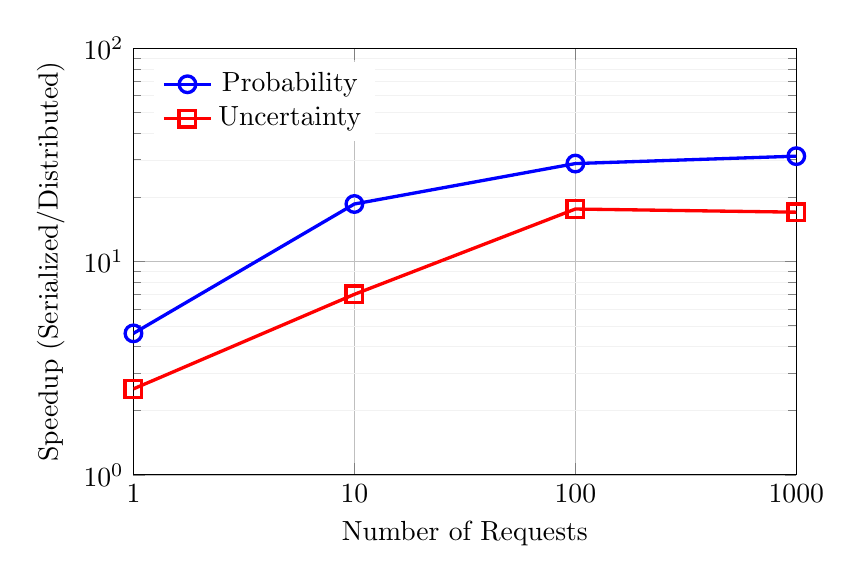
\begin{tikzpicture}
        \begin{loglogaxis}[
            width=10cm,
            height=7cm,
            grid=both,
            minor grid style={line width=.1pt, draw=gray!10},
            major grid style={line width=.2pt, draw=gray!50},
            xlabel={Number of Requests},
            ylabel={Speedup (Serialized/Distributed)},
            legend pos=north west,
            legend style={draw=none},
            xtick={1,10,100,1000},
            xticklabels={1,10,100,1000},
            log basis x=10,
            log basis y=10,
            ymin=1, ymax=100,
            xmin=1, xmax=1000
            ]
            
            % Probability speedup data
            \addplot[
                color=blue,
                mark=o,
                line width=1.2pt,
                mark size=3pt
                ] coordinates {
                (1, 4.603)
                (10, 18.6)
                (100, 28.776)
                (1000, 31.167)
            };
            
            % Uncertainty speedup data
            \addplot[
                color=red,
                mark=square,
                line width=1.2pt,
                mark size=3pt
                ] coordinates {
                (1, 2.528)
                (10, 7.016)
                (100, 17.616)
                (1000, 17.029)
            };
            
            \legend{Probability, Uncertainty}
        \end{loglogaxis}
    \end{tikzpicture}
    \caption{Speedup comparison between serialized and distributed execution for different request volumes.}
    \label{fig:speedup}
\end{figure}

The super-linear speedup for single request workloads is caused by the elimination of I/O processes. In the serialized \texttt{scram-cli} baseline, each run must (i) parse command-line arguments, (ii) read and validate the input XML fault-tree, (iii) launch a new process to execute the solver, and (iv) synchronously write results back to disk. In the distributed implementation, the request payload already contains the model and run-time parameters, which are passed directly to a Node.js native addon that invokes the underlying \texttt{scram} library. Result persistence is off-loaded to an asynchronous database writing process. So, both the initial XML parsing and the final file output are effectively removed from the process. Consequently, execution time reflects only the core solver computation, producing the observed speed-ups ($S\approx4.6$ for probability estimation and $S\approx2.5$ for uncertainty analysis) even at a single concurrent request.  
Beyond 100 jobs, speed-up saturates owing to:

\begin{itemize}
  \item \textbf{Worker saturation}: eight containers fully occupy the host’s 8 hardware threads; adding jobs only increases wait time.
  \item \textbf{Queue latency}: larger batches incur longer residence times in RabbitMQ prior to dispatch.
  \item \textbf{Memory bandwidth limits}: uncertainty calculations are memory-bound; waiting time grows with concurrency.
\end{itemize}

These findings validate that the combined architecture of Docker-Swarm and RabbitMQ delivers near-linear scaling for practical PRA workloads up to the tested concurrency and provides an order-of-magnitude reduction in wall-clock time compared with serialized execution.
}

% \section{Handling Multi-Hazard Models in Parallel}
% \subsection{Integration of Hazard Modules}
% \subsection{Numerical Stability and Overflow Handling}

% \section{Security and Data Ownership}
% \subsection{Data Sharing Protocols}
% \subsection{Access Control and Regulatory Constraints}